\subsubsection{并集}

已知方程 $x^2 - 4 = 0$ 的解集为
$$A = \{2,\ -2\}\text{,}$$
方程 $x^2 - 1 = 0$ 的解集为
$$B = \{1,\ -1\}\text{,}$$
那么方程
$$(x^2 - 4)(x^2 - 1) = 0$$
的解集为
$$\{1,\ -1,\ 2,\ -2\}\text{。}$$

容易看出,集合$\{1,\ -1,\ 2,\ -2\}$是由所有属于$A$或属于$B$的元素所组成的。

一般地,由所有属于集合$A$或属于集合$B$的元素所组成的集合,叫做$A$,$B$的\textbf{并集},记作$A \cup B$(可读作“$A$并$B$”),即
$$A \cup B = \{ x \mid x \in A \text{,或} x \in B \}\text{。}$$

这样,方程$(x^2 - 4)(x^2 - 1) = 0$ 的解集,可以从求方程 $x^2 - 4 = 0$ 的解集与方程 $x^2 - 1 = 0$ 的解集的并集而得到,即
$$\{ 2,\ -2\} \cup \{ 1,\ -1\}  = \{ 1,\ -1,\ 2,\ -2\} \text{。}$$

\begin{figure}[htbp]
    \centering
    \begin{minipage}{7cm}
    \centering
    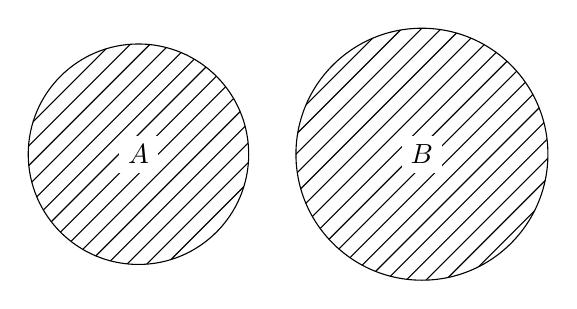
\begin{tikzpicture}
        \coordinate (A) at (0,0);
        \coordinate (B) at (3.6,0);
        \draw (A) circle (1.4);
        \draw (B) circle (1.6);
        \begin{scope}
            \clip (A) circle (1.4);
            \foreach \x in {-2,-1.75,...,2}
            \draw[xshift=\x cm] (2,2)--(-2,-2);
        \end{scope}
        \begin{scope}
            \clip (B) circle (1.6);
            \foreach \x in {-2,-1.75,...,2.25}
            \draw[xshift=3.5cm +\x cm]  (2,2)--(-2,-2);
        \end{scope}
        \node at (A) [fill=white] {$A$};
        \node at (B) [fill=white] {$B$};
    \end{tikzpicture}
    \caption*{(1)}
    \end{minipage}
    \qquad
    \begin{minipage}{8cm}
    \centering
    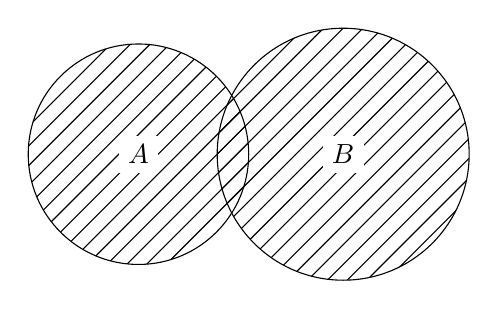
\begin{tikzpicture}
        \coordinate (A) at (0,0);
        \coordinate (B) at (2.6,0);
        \draw (A) circle (1.4);
        \draw (B) circle (1.6);
        \begin{scope}
            \clip (A) circle (1.4);
            \foreach \x in {-2,-1.75,...,2}
            \draw[xshift=\x cm] (2,2)--(-2,-2);
        \end{scope}
        \begin{scope}
            \clip (B) circle (1.6);
            \foreach \x in {-2,-1.75,...,2.25}
            \draw[xshift=2.5cm +\x cm]  (2,2)--(-2,-2);
        \end{scope}
        \node at (A) [fill=white] {$A$};
        \node at (B) [fill=white] {$B$};
    \end{tikzpicture}
    \caption*{(2)}
    \end{minipage}
    \caption{}\label{fig:1-3}
\end{figure}

图\ref{fig:1-3}中的阴影部分,表示集合$A$,$B$的并集$A \cup B$。

注意:我们已经知道,集合中的元素是没有重复现象的。因此,在求两个集合的并集时,这两个集合的公共元素在并集中只能出现一次。例如,设$A = \{3, 5, 6, 8\}$,$B = \{4, 5, 7, 8\}$,则$A \cup B$应是$\{3, 4, 5, 6, 7, 8\}$,而不是 $\{3, 5, 6, 8, 4, 5, 7, 8\}$。

由并集定义容易知道,对于任何集合$A$,$B$,有
\begin{gather*} 
    A \cup A = A, \quad A \cup \kongji = A , \\
    A \cup B = B \cup A \text{。}
\end{gather*}

\liti 设 $A = \{x \mid -1<x<2 \}$,$B= \{x \mid 1<x<3\}$,求$A \cup B$。

\jie
\begin{minipage}[t]{8cm}
    \gongshishangyi
    \begin{align*}
        A \cup B &= \{x \mid -1<x<2\} \cup \{x \mid 1<x<3\} \\
                 &= \{x \mid -1<x<3\} \text{。} \\
    \end{align*}
\end{minipage}

\liti 设 $A =\{\text{锐角三角形}\}$,$B=\{\text{钝角三角形}\}$,求$A \cup B$。

\jie
\begin{minipage}[t]{7cm}
    \gongshishangyi
    \begin{align*}
        A \cup B &= \{\text{锐角三角形}\} \cup \{\text{钝角三角形}\} \\
                 &= \{\text{锐角三角形,或钝角三角形}\} \\
                 &= \{\text{斜三角形}\} \text{。}
    \end{align*}
\end{minipage}

\liti 写出不等式 $x^2+x-6 \ge 0$ 的解集并进行化简。

\jie 不等式 $x^2+x-6 \ge 0$ 的解集是

\begin{minipage}{10cm}
    \begin{align*}
        \{ x \mid x^2+x-6 \ge 0\} &= \{ x \mid x \le -3 \} \cup \{ x \mid x \ge 2 \} \\
            &= \{ x \mid x \le -3 \text{,或} x \ge 2 \} \text{。}
    \end{align*}
\end{minipage}

\liti 设 $A = \left\{ x \,\middle|\,  -4 < x < -\dfrac 1 2\right\}$,$B = \{x \mid x \le -4\}$,求 $A \cup B$,$A \cap B$。

\jie
\begin{minipage}[t]{8cm}
    \begin{align*}
        A \cup B &= \left\{ x \,\middle|\,  -4 < x < -\dfrac 1 2\right\} \cup \{x \mid x \le -4\} \\
                 &= \left\{ x \,\middle|\,  x < -\dfrac 1 2\right\}, \\
        A \cap B &= \left\{ x \,\middle|\,  -4 < x < -\dfrac 1 2\right\} \cap \{x \mid x \le -4\} \\
                 &= \kongji \text{。}
    \end{align*}
\end{minipage}

\liti 已知 $Q$ 为有理数集,$Z$ 为整数集,求 $Q \cup Z$,$Q \cap Z$。

\jie
\begin{minipage}{8cm}
    \begin{align*}
        Q \cup Z &= \{\text{有理数}\} \cup \{\text{整数}\} = \{\text{有理数}\} = Q ,\\
        Q \cap Z &= \{\text{有理数}\} \cap \{\text{整数}\} = \{\text{整数}\} = Z \text{。}
    \end{align*}
\end{minipage}
